% !TEX root = ../XJ_thesis.tex
%
\chapter{A Trilateral Weighted Sparse Coding Scheme for Realistic Image Denoising}
\label{sec:internalsc}


\section{Introduction}

Image denoising aims to recover the clean image $\bm{x}$ from its noisy observation $\bm{y}=\bm{x}+\bm{n}$, where $\bm{n}$ is the corrupted noise. The denoising problem has been extensively studied in computer vision and machine learning, and numerous statistical image modeling and learning methods have been proposed in the past decades \cite{ksvd,bm3d,cbm3d,lssc,ncsr,wnnm,epll,pgpd,mlp,csf,tnrd,dncnn,
Liu2008,noiseclinic,Zhu_2016_CVPR,crosschannel2016,neatimage}. Most of the existing methods \cite{ksvd,bm3d,cbm3d,lssc,ncsr,wnnm,epll,pgpd,mlp,csf,tnrd,dncnn} focus on additive white Gaussian noise (AWGN), which can be categorized into dictionary learning based methods \cite{ksvd}, nonlocal self-similarity based methods \cite{bm3d,cbm3d,lssc,ncsr,wnnm}, sparsity based methods \cite{ksvd,bm3d,cbm3d,lssc,ncsr}, low-rankness based methods \cite{wnnm}, generative learning based methods \cite{epll,pgpd}, and discriminative learning based methods \cite{mlp,csf,tnrd,dncnn}. However, the realistic noise in real-world images is much more complex than AWGN \cite{crosschannel2016} and varies with different cameras and camera settings (such as ISO, shutter speed, and aperture, etc.). Though have shown promising performance on AWGN noise removal, the above methods \cite{ksvd,bm3d,cbm3d,lssc,ncsr,wnnm,epll,pgpd,mlp,csf,tnrd,dncnn} will become much less effective when dealing with complex realistic noise.

In the past decade, several denoising methods for realistic noisy images have been developed \cite{cbm3d,Liu2008,noiseclinic,Zhu_2016_CVPR,
crosschannel2016,neatimage}. Among them, CBM3D \cite{cbm3d} is a representative method which applies the benchmark BM3D method \cite{bm3d} to each channel of the luminance-chrominance space of the noisy image. Liu et al. \cite{Liu2008} proposed to estimate the noise via a ``noise level function'' and remove the noise for each channel of the real image. However, processing each channel separately would often achieve unsatisfactory performance and generate artifacts. The methods \cite{noiseclinic,Zhu_2016_CVPR} perform image denoising by concatenating the patches of RGB channels into a vector. However, the concatenation does not consider the different noise statistics among different channels. The method in \cite{crosschannel2016} models the noise in a noisy image as multivariate Gaussian and performs denoising by the Non-local Bayes filter \cite{noiseclinic}. The commercial software Neat Image \cite{neatimage} estimates the global noise parameters from a flat region of the given noisy image and filters the noise accordingly. However, both the two methods \cite{crosschannel2016,neatimage} ignore the local statistical property of the noise which is signal dependent and varies in different pixels. By far, realistic image denoising remains a challenging problem in low level vision.  

Sparse coding (SC) \cite{lasso} has been well studied in many computer vision and learning problems \cite{src,yang2010image}, including image denoising \cite{ksvd,lssc,ncsr}. Usually, the SC models employ an $\ell_{2}$ (or Frobenious) norm to describe the residual in the data term, and minimize an energy function 
$
\min_{\bm{\alpha}}
\|
\bm{y}-\bm{D}\bm{\alpha}
\|_{2}^{2}
+
\mathcal{R}(\bm{\alpha})
$, where $\bm{D}$ is the dictionary, $\bm{\alpha}$ is the sparse coefficients vector of signal $\bm{y}$, and $\mathcal{R}(\bm{\alpha})$ is usually the $\ell_{0}$ or $\ell_{1}$ norm of $\bm{\alpha}$ to enforce sparse regularization. Some representative SC based image denoising methods include K-SVD \cite{ksvd}, LSSC \cite{lssc}, and NCSR \cite{ncsr}. Though being effective on dealing with AWGN, SC based denoising methods are essentially limited by the $\ell_{2}$ (or Frobenious) norm based data term, which actually assumes white Gaussian noise and is not able to characterize the complex realistic noise. Recently, there are several methods \cite{Zhu_2016_CVPR,zhao2014robust} modeling complex noise via mixture of Gaussian distribution. However, these methods \cite{Zhu_2016_CVPR,zhao2014robust} are time-consuming due to employing variational Bayesian inference techniques.

In this work, we propose to lift the SC model to a robust denoiser for real noisy images by utilizing the channel-wise statistics and locally signal dependent property of the realistic noise. Specifically, we propose a trilateral weighted sparse coding (TWSC) scheme for realistic image denoising. Two weight matrices are introduced into the data term of the SC model to characterize the realistic noise property, and another weight matrix is introduced into the regularization term to characterize the sparsity priors of natural images. To solve the proposed TWSC model, we reformulate it into a linear equality-constrained optimization program, which can be minimized under the alternating direction method of multipliers \cite{admm} framework. Theoretical analysis on the existence and uniqueness of the solution of the TWSC model, as well as the convergence of the algorithm, are presented. Experiments on real noisy image datasets demonstrate that the proposed TWSC method achieves much more robust realistic denoising performance than the existing methods.





\section{The Proposed Realistic Image Denoising Algorithm}

\subsection{The Trilateral Weighted Sparse Coding Model}

Denote by $\bm{y}_{c}=\bm{x}_{c}+\bm{n}_{c}$ the noisy observation of the clean color image $\bm{x}_{c}$, where $c\in\{r, g, b\}$ is the index of R, G, B channels and $\bm{n}_{c}$ is the noise in channel $c$.\ A local patch of size $p\times p \times 3$ is extracted from the image and stretched to a vector, denoted by $\bm{y}=[\bm{y}_{r}^{\top}\ \bm{y}_{g}^{\top}\ \bm{y}_{b}^{\top}]^{\top}\in\mathbb{R}^{3p^{2}}$, where $\bm{y}_{c}\in\mathbb{R}^{p^{2}}$ is the corresponding patch in channel $c$.\ For each local patch $\bm{y}$, we search the $M$ most similar patches to it (including $\bm{y}$ itself) by Euclidean distance in a local window around it.\ By stacking the $M$ similar patches column by column, we form a noisy patch matrix $\bm{Y}=\bm{X}+\bm{N}\in\mathbb{R}^{3p^{2}\times M}$, where $\bm{X}$ and $\bm{N}$ are the corresponding clean and noise patch matrices, respectively.\ The noisy patch matrix can be written as $\bm{Y}=[\bm{Y}_{r}^{\top}\ \bm{Y}_{g}^{\top}\ \bm{Y}_{b}^{\top}]^{\top}$, where $\bm{Y}_{c}$ is the sub-matrix of channel $c$.\ 

Suppose that we have a dictionary $\bm{D}=[\bm{D}_{r}^{\top}\ \bm{D}_{g}^{\top}\ \bm{D}_{b}^{\top}]^{\top}$, where $\bm{D}_{c}$ is the sub-dictionary corresponding to channel $c$.\ Under the sparse coding (SC) framework \cite{lasso}, the sparse code matrix of $\bm{Y}$ over $\bm{D}$ can be obtained by
\begin{equation}
\label{equ5-1}
\hat{\bm{C}}
=
\arg\min\nolimits_{\bm{C}}
\|\bm{Y}-\bm{D}\bm{C}\|_{F}^{2}
+
\lambda\|\bm{C}\|_{1},
\end{equation}
where $\lambda$ is the regularization parameter. Once $\hat{\bm{C}}$ is computed,
the latent clean patch matrix $\hat{\bm{X}}$ can be estimated as $\hat{\bm{X}}=\bm{D}\hat{\bm{C}}$.\ In this work, we use an adaptive dictionary to the given data matrix $\bm{Y}$. The dictionary $\bm{D}$ can be obtained by applying SVD to $\bm{Y}$ as 
\begin{equation}
\label{equ5-2}
\bm{Y} =\bm{D}\bm{S}\bm{V}^{\top}.
\end{equation}
% $\bm{Y}_{c} =\bm{D}_{c}\bm{S}_{c}\bm{V}_{c}^{\top}$ for $c\in\{r,g,b\}$.
Though SC based methods \cite{ksvd,lssc,ncsr} have achieved promising performance in removing additive white Gaussian noise (AWGN), their performance is very limited when dealing with realistic noise in real-world images. The reason is that the realistic noise is non-Gaussian, varies locally and across channels, which cannot be characterized well by the Frobenious norm in model (\ref{equ5-1}).  

To account for the varying statistics of the realistic noise in different channels and different patches, we introduce two weight matrices $\bm{W}_{1}\in\mathbb{R}^{3p^2\times3p^2}$ and $\bm{W}_{2}\in\mathbb{R}^{M\times M}$ to characterize the SC residual ($\bm{Y}-\bm{D}\bm{C}$) in the data term of Eq.\ (\ref{equ5-1}). Besides, to better characterize the sparse priors of the natural images, we introduce a third weight matrix $\bm{W}_{3}$, which is related to the distribution of the sparse coefficients matrix $\bm{C}$, into the regularization term of Eq.\ (\ref{equ5-1}). Finally, the proposed trilateral weighted sparse coding (TWSC) model is formulated as follows:
\begin{equation}
\label{equ5-3}
\min\nolimits_{\bm{C}}\|\bm{W}_{1}(\bm{Y}-\bm{D}\bm{C})\bm{W}_{2}\|_{F}^{2}
+
\|\bm{W}_{3}^{-1}\bm{C}\|_{1}.
\end{equation}
All the three weight matrices are diagonal matrices and have clear physical meanings. $\bm{W}_{1}$ is a block diagonal matrix. Each block of $\bm{W}_{1}$ has the same diagonal elements to describe the noise properties in each RGB channel. The realistic noise in a local region could be approximately modeled as Gaussian \cite{Leungtip}, and each diagonal element of weight matrix $\bm{W}_{2}$ is used to describe the noise variance in each patch $\bm{y}$. Geometrically speaking, $\bm{W}_{1}$ is employed to regularize the row discrepancy of residual matrix ($\bm{Y}-\bm{D}\bm{C}$), while $\bm{W}_{2}$ is employed to regularize the column discrepancy of ($\bm{Y}-\bm{D}\bm{C}$). For matrix $\bm{W}_{3}$, each diagonal element will be set based on the prior information on $\bm{C}$. All the three weight matrices $\bm{W}_{1},\bm{W}_{2},\bm{W}_{3}$ can be determined under the \textsl{maximum a-posterior} (MAP) estimation framework, as described in detail in the next subsection. 

 
\subsection{The Setting of Weight Matrices}

We determine the weight matrices $\bm{W}_{1},\bm{W}_{2},\bm{W}_{3}$ by employing the MAP estimation:

\begin{equation}
\label{equ5-4}
\hat{\bm{C}} 
=
\arg\max\nolimits_{\bm{C}}\ln P(\bm{C}|\bm{Y})
=
\arg\max\nolimits_{\bm{C}}\{\ln P(\bm{Y}|\bm{C})+\ln P(\bm{C})\}.
\end{equation}
The log-likelihood term $\ln P(\bm{Y}|\bm{C})$ is characterized by the
statistics of noise or residual.\ According to \cite{Leungtip}, it can be assumed that the noise is independently and identically distributed (i.i.d.) in each channel and each patch with Gaussian distribution. We denote by $\sigma_{c}$ the standard deviation (std) of noise in channel $c$, $c\in\{r,g,b\}$, and denote by $\sigma_{m}$ the std of noise in a color patch $m$, $m\in\{1,...,M\}$. Denote by $\sigma_{cm}$ the noise std of sub-patch $m$ in channel $c$. Then we have:

\begin{equation}
\label{equ5-5}
P(\bm{Y}|\bm{C}) 
= 
\prod\nolimits_{c\in\{r, g, b\}}
\prod\nolimits_{m=1}^{M}
(\pi\sigma_{cm})^{-p^{2}}
\exp(-\sigma_{cm}^{-2}\|\bm{y}_{cm}-\bm{D}_{c}\bm{c}_{m}\|_{2}^{2}),
\end{equation}
where $\bm{y}_{cm},\bm{c}_{m}$ are the $m$th column of the matrices $\bm{Y}_{c}$ and $\bm{C}$, respectively. From the perspective of statistics \cite{glm}, the set of $\{\sigma_{cm}\}$ can be viewed as a $3\times M$ contingency table created by two variables $\sigma_{c}$ and $\sigma_{m}$, and their relationship could be modeled by a log-linear model $\sigma_{cm}=\sigma_{c}^{l_{1}}\sigma_{m}^{l_{2}}$, where $l_{1}+l_{2}=1$. The estimation of $\{\sigma_{cm}\}$ can be reduced to the estimation of $\{\sigma_{c}\}$ and $\{\sigma_{m}\}$. Specifically, the noise std $\sigma_{c}$ of channel $c$ can be estimated by some noise estimation methods \cite{Chen2015ICCV}. The noise std for the $m$th patch of $\bm{Y}$ can be initialized as 
$
\sigma_{m}=\sigma\triangleq \sqrt{(\sigma_{r}^{2}+\sigma_{g}^{2}+\sigma_{b}^{2})/3}
$
and updated as $\sigma_{m}=\sqrt{\sigma^2-\|\bm{y}_{m}-\bm{x}_{m}\|_{2}^{2}}$, where $\bm{y}_{m}$ is the $m$th image patch in $\bm{Y}$, and $\bm{x}_{m}=\bm{D}\bm{c}_{m}$ is the $m$th image patch recovered in previous iteration (refer to Algorithm 2 in next section).\

We assume that each column $\bm{c}_{m}$ of coefficients matrix $\bm{C}$ follows i.i.d. Laplacian distribution. Specifically, for each entry $\bm{c}_{m}^{i}$, which is the coding coefficient of the $m$th patch over the $i$th atom of dictionary $\bm{D}$, we assume that it follows distribution  $(2\bm{S}_{i})^{-1}\exp(-\bm{S}_{i}^{-1}|\bm{c}_{m}^{i}|)$, where $\bm{S}_{i}$ is the $i$th element of the diagonal singular value matrix $\bm{S}$ in Eq.\ (\ref{equ5-2}). Note that we set the scale factor of the distribution as the inverse of the $i$th singular value $\bm{S}_{i}$. This is because the larger the singular value $\bm{S}_{i}$ is, the more important the $i$th singular vector in $\bm{D}$ should be, and hence the distribution of the coding coefficients over this singular vector should have stronger regularization with less sparse distribution. The prior term in Eq.\ (\ref{equ5-4}) becomes
\begin{equation}
\label{equ5-6}
P(\bm{C})
=
\prod\nolimits_{m=1}^{M}
\prod\nolimits_{i=1}^{3p^{2}}
(2\bm{S}_{i})^{-1}\exp(-\bm{S}_{i}^{-1}|\bm{c}_{m}^{i}|).
\end{equation}


Put (\ref{equ5-6}) and (\ref{equ5-5}) into (\ref{equ5-4}) and consider the log-linear model $\sigma_{cm}=\sigma_{c}^{l_{1}}\sigma_{m}^{l_{2}}$, we have

\begin{equation}
\label{equ5-7}
\begin{split}
\hat{\bm{C}}
&
=
\arg\min\nolimits_{\bm{C}}
\sum\nolimits_{c\in\{r, g, b\}}
\sum\nolimits_{m=1}^{M}
\sigma_{cm}^{-2}
\|(\bm{y}_{cm}-\bm{D}_{c}\bm{c}_{m})\|_{2}^{2}
+
\sum\nolimits_{m=1}^{M}
\|\bm{S}^{-1}\bm{c}_{m}\|_{1}
\\
&
=
\arg\min\nolimits_{\bm{C}}
\sum\nolimits_{c\in\{r, g, b\}}
\sigma_{c}^{-2l_{1}}
\|(\bm{Y}_{c}-\bm{D}_{c}\bm{C})\bm{W}_{2}\|_{F}^{2}+\|\bm{S}^{-1}\bm{C}\|_{1}
\\
&
=
\arg\min\nolimits_{\bm{C}}\|\bm{W}_{1}(\bm{Y}-\bm{D}\bm{C})\bm{W}_{2}\|_{F}^{2}+\|\bm{W}_{3}^{-1}\bm{C}\|_{1},
\end{split}
\end{equation}
where
\begin{equation}
\label{equ5-8}
\bm{W}_{1}
=
\text{diag}(\sigma_{r}^{-l_{1}}\bm{I}_{p^2},\sigma_{g}^{-l_{1}}\bm{I}_{p^2},\sigma_{b}^{-l_{1}}\bm{I}_{p^2})
,
\bm{W}_{2}
=
\text{diag}(\sigma_{1}^{-l_{2}},...,\sigma_{M}^{-l_{2}})
,
\bm{W}_{3} 
= 
\bm{S}
,
\end{equation}
and $\bm{I}_{p^2}$ is the $p^{2}$ dimensional identity matrix. We can see that the diagonal elements of $\bm{W}_{1}$ and $\bm{W}_{2}$ are determined by the noise standard deviation in each channel and each patch, respectively. The stronger the noise in a channel and a patch, the less the contribution that channel and patch will make to the denoising output. In our experiments, we consider $\{\sigma_{c}\}, \{\sigma_{m}\}$ of equal importance and empirically set $l_{1}=l_{2}=0.5$.



\subsection{Model Optimization}

Letting $\bm{C}^{*}=\bm{W}_{3}^{-1}\bm{C}$, we can transfer the weight matrix $\bm{W}_{3}$ into the data term of (\ref{equ5-3}). Thus, the TWSC model (\ref{equ5-3}) is reformulated as 
\begin{equation}
\label{equ5-9}
\min\nolimits_{\bm{C}^{*}}\|\bm{W}_{1}(\bm{Y}-\bm{D}\bm{W}_{3}\bm{C}^{*})\bm{W}_{2}\|_{F}^{2}
+
\|\bm{C}^{*}\|_{1}.
\end{equation}
To make the notation simple, we remove the superscript $*$ in $\bm{C}^{*}$ and still use $\bm{C}$ in the following development.

Since the problem (\ref{equ5-9}) is convex, we can obtain its globally optimal solution. We employ the variable splitting method \cite{Eckstein1992} to solve it.\ By introducing an augmented variable $\bm{Z}$, the problem (\ref{equ5-9}) is reformulated as a linear equality-constrained problem with two variables $\bm{C}$ and $\bm{Z}$:
\begin{equation}
\label{equ5-10}
\min\nolimits_{\bm{C},\bm{Z}}\|\bm{W}_{1}(\bm{Y}-\bm{D}\bm{W}_{3}\bm{C})\bm{W}_{2}\|_{F}^{2}
+
\|\bm{Z}\|_{1}
\quad
\text{s.t.}
\quad
\bm{C}=\bm{Z}.
\end{equation}
Since the objective function is separable w.r.t. the two variables, the problem (\ref{equ5-10}) can be solved under the alternating direction method of multipliers (ADMM) \cite{admm} framework.\ The augmented Lagrangian function is:
\begin{equation}
\label{equ5-11}
\begin{split}
\mathcal{L}(\bm{C},\bm{Z},\bm{\Delta},\rho)
=
&\|\bm{W}_{1}(\bm{Y}-\bm{D}\bm{W}_{3}\bm{C})\bm{W}_{2}\|_{F}^{2}
+
\|\bm{Z}\|_{1}
+
\langle
\bm{\Delta},\bm{C}-\bm{Z}
\rangle
+
\frac{\rho}{2}
\|\bm{C}-\bm{Z}\|_{F}^{2},
\end{split}
\end{equation}
where $\bm{\Delta}$ is the augmented Lagrangian multiplier and $\rho>0$ is the penalty parameter.\ We initialize the matrix variables $\bm{C}_{0}$, $\bm{Z}_{0}$, and $\bm{\Delta}_{0}$ to be comfortable zero matrix and $\rho_{0}>0$.\ Denote by ($\bm{C}_{k}, \bm{Z}_{k}$) and $\bm{\Delta}_{k}$ the optimization variables and Lagrange multiplier at iteration $k$ ($k=0,1,2,...$), respectively.\ By taking derivatives of the Lagrangian function $\mathcal{L}$ w.r.t. $\bm{C}$ and $\bm{Z}$ and setting the derivatives to be zeros, we can alternatively update the variables as follows:
\\
(1) \textbf{Update $\bm{C}$ by fixing $\bm{Z}$ and $\bm{\Delta}$}:
\begin{equation}
\label{equ5-12}
\bm{C}_{k+1}
=
\arg\min\nolimits_{\bm{C}}
\|\bm{W}_{1}(\bm{Y}-\bm{D}\bm{W}_{3}\bm{C})\bm{W}_{2}\|_{F}^{2} 
+
\frac{\rho_{k}}{2}\|\bm{C} - \bm{Z}_{k} + \rho_{k}^{-1}\bm{\Delta}_{k}||_{F}^{2}.
\end{equation}
This is a two-sided weighted least squares regression problem with the solution satisfying that
\begin{equation}
\label{equ5-13}
\bm{A}\bm{C}_{k+1}
+
\bm{C}_{k+1}\bm{B}_{k}
=
\bm{E}_{k},
\end{equation}
where $\bm{A}=\bm{W}_{3}^{\top}\bm{D}^{\top}\bm{W}_{1}^{\top}\bm{W}_{1}\bm{D}\bm{W}_{3}$, $\bm{B}_{k}=\frac{\rho_{k}}{2}(\bm{W}_{2}\bm{W}_{2}^{\top})^{-1}$, and $\bm{E}_{k}=\bm{W}_{3}^{\top}\bm{D}^{\top}\bm{W}_{1}^{\top}\bm{W}_{1}\bm{Y}+(\frac{\rho_{k}}{2}\bm{Z}_{k} -\frac{1}{2}\bm{\Delta}_{k})(\bm{W}_{2}\bm{W}_{2}^{\top})^{-1}$. Eq.\ (\ref{equ5-13}) is a standard Sylvester equation (SE) which has a unique solution if and only if $\sigma(\bm{A})\cap\sigma(-\bm{B}_{k})=\emptyset$, where $\sigma(\bm{F})$ denotes the spectrum, i.e., the set of eigenvalues, of the matrix $\bm{F}$ \cite{simoncini2016computational}. We can rewrite the SE (\ref{equ5-13}) as 
\begin{equation}
\label{equ5-14}
(\bm{I}_{M}\otimes\bm{A}
+
\bm{B}_{k}^{\top}\otimes\bm{I}_{3p^2})\text{vec}(\bm{C}_{k+1})
=
\text{vec}(\bm{E}_{k}),
\end{equation}
and the solution $\bm{C}_{k+1}$ (if existed) can be obtained via $\bm{C}_{k+1}=\text{vec}^{-1}(\text{vec}(\bm{C}_{k+1}))$, where $\text{vec}^{-1}(\bullet)$ is the inverse of the vec-operator $\text{vec}(\bullet)$.
Detailed theoretical analysis on the existence of the unique solution is given in Section 3.
\\
(2) \textbf{Update $\bm{Z}$ by fixing $\bm{C}$ and $\bm{\Delta}$}:
\begin{equation}
\label{equ5-15}
\bm{Z}_{k+1}
=
\arg\min\nolimits_{\bm{Z}}\frac{\rho_{k}}{2}
\|\bm{Z} - (\bm{C}_{k+1}+\rho_{k}^{-1}\bm{\Delta}_{k})\|_{F}^{2}
+
\|\bm{Z}\|_{1}.
\end{equation}
This problem has a closed-form solution as 
\begin{equation}
\label{equ5-16}
\bm{Z}_{k+1}
=
\mathcal{S}_{\rho_{k}^{-1}}(\bm{C}_{k+1}+\rho_{k}^{-1}\bm{\Delta}_{k}),
\end{equation}
where $\mathcal{S}_{\lambda}(x) = \text{sign}(x)\max(x-\lambda, 0)$ is the soft-thresholding operator.
\\
(3) \textbf{Update $\bm{\Delta}$ by fixing $\bm{X}$ and $\bm{Z}$}:
\begin{equation}
\label{equ5-17}
\bm{\Delta}_{k+1}
=
\bm{\Delta}_{k} + \rho_{k}(\bm{C}_{k+1}-\bm{Z}_{k+1}).
\end{equation}
(4) \textbf{Update $\rho$}: $\rho_{k+1}= \mu\rho_{k}$, where $\mu>1$.

The above alternative updating steps are repeated until the convergence condition is satisfied or the number of iterations exceeds a preset threshold $K_{1}$.\ The ADMM algorithm converges when $\|\bm{C}_{k+1}-\bm{Z}_{k+1}\|_{F}\le \text{Tol}$, $\|\bm{C}_{k+1}-\bm{C}_{k}\|_{F}\le \text{Tol}$, and $\|\bm{Z}_{k+1}-\bm{Z}_{k}\|_{F}\le \text{Tol}$ are simultaneously satisfied, where $\text{Tol}>0$ is a small tolerance number.\ We summarize the updating procedures in Algorithm 1.\ The convergence analysis of Algorithm 1 is given in Theorem \ref{th5-1}.\ Note that here we employ an unbounded sequence of $\{\rho_{k}\}$, i.e., $\lim_{k \to \infty} \rho_{k}=+\infty$, to make sure that Algorithm 1 converges. In fact, since the optimization problem (\ref{equ5-10}) is convex, it is naturally convergent under the ADMM \cite{admm} framework.


\subsection{Convergence Analysis}


\begin{theorem}
\label{th5-1}
Given $\rho_{k+1}=\mu\rho_{k}$ ($\rho_{0}>0$) for $k\ge0$ and $\mu>1$, the sequences $\{\bm{C}_{k}\}$ and $\{\bm{Z}_{k}\}$ generated in Algorithm 1 satisfy:
\begin{align}
&
(a)\ 
\|\bm{C}_{k+1}-\bm{Z}_{k+1}\|_{F}=\mathcal{O}(\rho_{k}^{-1})
\ 
\textsl{as}\ k \to +\infty
,\ 
\textsl{i.e.},\ 
\lim_{k \to +\infty} \|\bm{C}_{k+1}-\bm{Z}_{k+1}\|_{F}=0;
\\
&
(b)\ 
\textsl{If}\ 
\|\bm{Z}_{k+1}-\bm{Z}_{k}\|_{F}=\mathcal{O}(\rho_{k}^{-1})
\ 
\textsl{as}\ k \to +\infty
,\ 
\textsl{then} 
\lim_{k \to +\infty} \|\bm{C}_{k+1}-\bm{C}_{k}\|_{F}=0;
\\
&
(c)\ 
\textsl{If}\ 
\lim_{k \to +\infty} \|\bm{C}_{k+1}-\bm{C}_{k}\|_{F}=0
,\ 
\textsl{then} 
\lim_{k \to +\infty} \|\bm{Z}_{k+1}-\bm{Z}_{k}\|_{F}=0.
\end{align}
\end{theorem}
The proof of Theorem \ref{th5-1} can be found in the supplementary file.\ Though Theorem \ref{th5-1} could not directly guarantee $\lim_{k \to +\infty}\|\bm{C}_{k+1}-\bm{C}_{k}\|_{F}=0$ and $\lim_{k \to +\infty}\|\bm{Z}_{k+1}-\bm{Z}_{k}\|_{F}=0$, it is empirically found that both $\|\bm{C}_{k+1}-\bm{C}_{k}\|_{F}$ and $\|\bm{Z}_{k+1}-\bm{Z}_{k}\|_{F}$ will approach to $0$ simultaneously in all our tests. In Figure \ref{fig5-1}, we can see that the maximal errors in $|\bm{C}_{k+1}-\bm{Z}_{k+1}|,|\bm{C}_{k+1}-\bm{C}_{k}|,|\bm{Z}_{k+1}-\bm{Z}_{k}|$ approach to $0$ simultaneously in 50 iterations.


\begin{table}[htb]
\centering
\begin{tabular}{l}
\hline
\textbf{Algorithm 1}: Solve Eq.\ (\ref{equ5-10}) via ADMM
\\
\hline
\textbf{Input:} $\bm{Y},\bm{W}_{1},\bm{W}_{2},\bm{W}_{3}$, $\mu$, $\text{Tol}$, $K_{1}$;
\\
\textbf{Initialization:} $\bm{C}_{0}=\bm{Z}_{0}=\bm{\Delta}_{0}=\bm{0}$, $\rho_{0}>0$, \text{T} = \text{False}, $k=0$; 
\\
\textbf{While} (\text{T} == \text{false}) \textbf{do}
\\
1. Update $\bm{C}_{k+1}$ by solving Eq.\ (\ref{equ5-13});
\\
2. Update $\bm{Z}_{k+1}$ by soft thresholding (\ref{equ5-16});
\\
3. Update $\bm{\Delta}_{k+1}$ as
$
\bm{\Delta}_{k+1}
=
\bm{\Delta}_{k} + \rho_{k}(\bm{C}_{k+1}-\bm{Z}_{k+1})
$;
\\
4. Update $\rho_{k+1}= \mu \rho_{k}$;
\\
5. $k \leftarrow k + 1$;
\\
\quad \textbf{if} (Converged) or ($k\ge K_{1}$)
\\
6.\quad \text{T} $\leftarrow$ \text{True}
\\
\quad \textbf{end if}
\\
\textbf{end while}
\\
\textbf{Output:} Matrices $\bm{C}$ and $\bm{Z}$.
\\
\hline
\end{tabular}
\end{table}


\begin{table}[htb]
\begin{tabular}{l}
\hline
\textbf{Algorithm 2}: Image Denoising by TWSC
\\
\hline
\textbf{Input:} Noisy image $\bm{y}_{c}$, $\{\sigma_{r}, \sigma_{g}, \sigma_{b}\}$, $K_{2}$;
\\
\textbf{Initialization:} $\hat{\bm{x}}_{c}^{(0)}=\bm{y}_{c}$, $\bm{y}_{c}^{(0)}=\bm{y}_{c}$;
\\
\textbf{for} $k = 1:K_{2}$ \textbf{do}
\\
1. Set $\bm{y}_{c}^{(k)}=\hat{\bm{x}}_{c}^{(k-1)}$;
\\
2. Extract local patches $\{\bm{y}_{j}\}_{j=1}^{N}$ from $\bm{y}_{c}^{(k)}$;
\\
\quad\textbf{for} each patch $\bm{y}_{j}$ \textbf{do}
\\
3.\quad Search nonlocal similar patches $\bm{Y}_{j}$;
\\
4.\quad Apply the TWSC model (\ref{equ5-3}) to $\bm{Y}_{j}$ and obtain the estimated $\bm{X}_{j}=\bm{D}\bm{C}$;
\\
\quad\textbf{end for}
\\
5. Aggregate $\{\bm{X}_{j}\}_{j=1}^{N}$ to form the image $\hat{\bm{x}}_{c}^{(k)}$;
\\
\textbf{end for}
\\
\textbf{Output:} Denoised image $\hat{\bm{x}}_{c}^{(K_{2})}$.
\\
\hline
\end{tabular}     
\end{table}

\begin{figure}[hbp]
\centering
\vspace{-81mm}
\raisebox{-0.15cm}{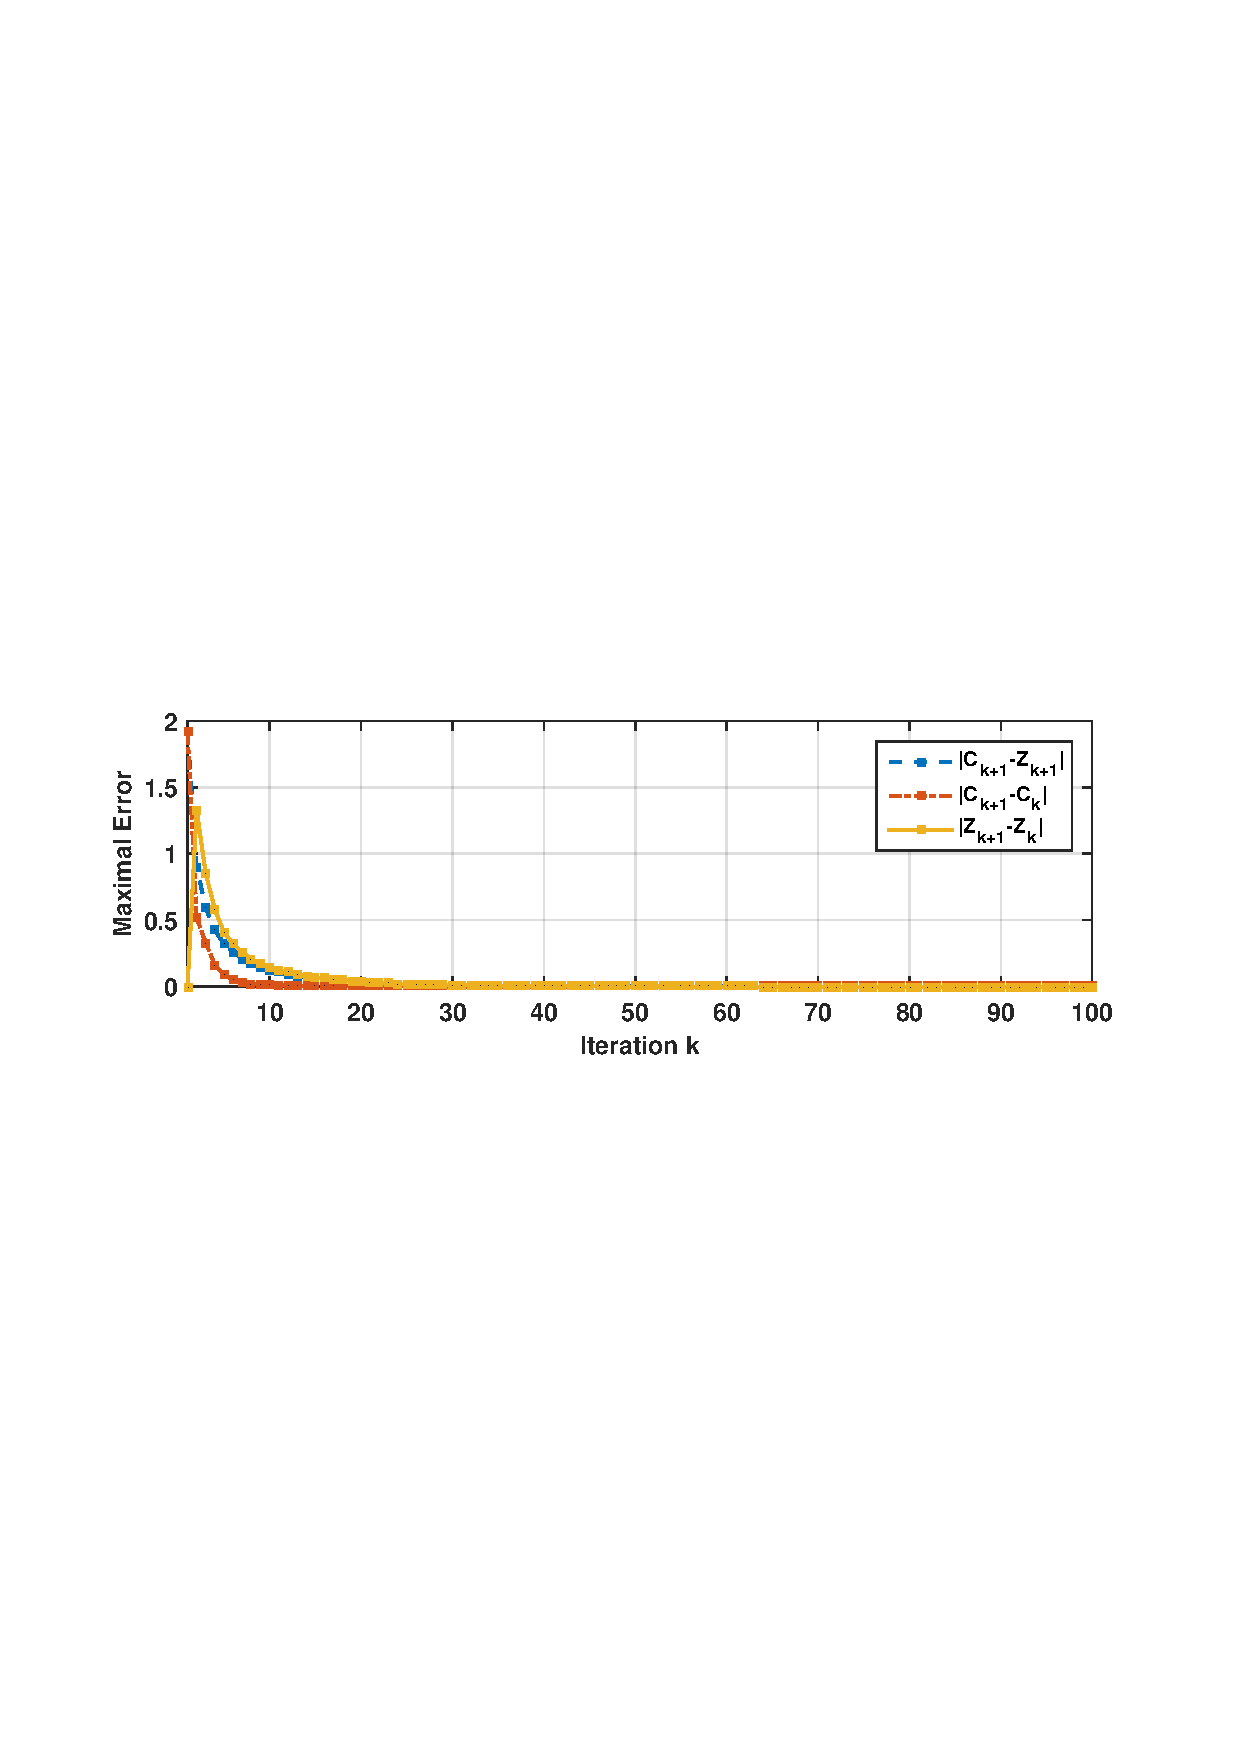
\includegraphics[width=1\textwidth]{images/twsc/LinearScaleConvergence.pdf}}
\vspace{-83mm}
\caption{The convergence curves of maximal errors in entries of $|\bm{C}_{k+1}-\bm{Z}_{k+1}|$ (blue line), $|\bm{C}_{k+1}-\bm{C}_{k}|$ (red line), and $|\bm{Z}_{k+1}-\bm{Z}_{k}|$ (yellow line). The test image is ``Barbara''.}
\label{fig5-1}
\end{figure}

\subsection{The Denoising Algorithm}

Given a noisy image $\bm{y}_{c}$, suppose that we have extracted $N$ local patches $\{\bm{y}_{j}\}_{j=1}^{N}$ and their similar patches.\ Then $N$ noisy patch matrices $\{\bm{Y}_{j}\}_{j=1}^{N}$ can be formed to estimate the clean matrices $\{\bm{X}_{j}\}_{j=1}^{N}$.\ The patches in matrices $\{\bm{X}_{j}\}_{j=1}^{N}$ are aggregated to form the denoised  image $\hat{\bm{x}}_{c}$.\ To obtain better denoising results, we perform the above denoising procedures for several iterations.\ The proposed TWSC based robust image denoising algorithm is summarized in Algorithm 2.


\section{Existence and Faster Solution of Sylvester Equation (\ref{equ5-13})}


The solution of the Sylvester equation (SE) (\ref{equ5-13}) does not always exist, though the solution is unique if it exists. Besides, solving SE (\ref{equ5-13}) is usually computationally expensive in high dimensional cases. In this section, we provide a sufficient condition to guarantee the existence of the solution to SE (\ref{equ5-13}), as well as a faster solution of (\ref{equ5-13}) to save the computational cost of Algorithms 1 and 2. 


\subsection{Existence of the Unique Solution}

Before we prove the existence of unique solution of Eq.\ (\ref{equ5-13}), we first introduce the following theorem. 

\begin{theorem}
\label{th5-2}
Assume that $\bm{A}\in\mathbb{R}^{3p^2\times 3p^2}$, $\bm{B}\in\mathbb{R}^{M\times M}$ are both symmetric and positive semi-definite matrices. If at least one of $\bm{A}, \bm{B}$ is positive definite, the Sylvester equation $\bm{A}\bm{C}
+
\bm{C}\bm{B}
=
\bm{E}$ has a unique solution for $\bm{C}\in \mathbb{R}^{3p^2\times M}$.
\end{theorem}

The proof of Theorem \ref{th5-2} can be found in the supplementary file. We then have the following corollary.

\begin{corollary}
The Sylvester equation (\ref{equ5-13}) has a unique solution.
\end{corollary}

\begin{proof}
Since $\bm{A},\bm{B}_{k}$ in (\ref{equ5-13}) are both symmetric and positive definite matrices, according to Theorem \ref{th5-2}, the SE (\ref{equ5-13}) has a unique solution. 
\end{proof}


\subsection{Faster Solution of the Sylvester Equation (\ref{equ5-13})}

The solution (\ref{equ5-14}) of the SE (\ref{equ5-13}) is typically obtained by the Bartels-Stewart algorithm \cite{Bartels1972}. This algorithm firstly employs a QR factorization \cite{GolubMatrix}, implemented via Gram-Schmidt process, to decompose the matrices $\bm{A}$ and $\bm{B}_{k}$ into Schur forms, and then solves the obtained triangular system by the back-substitution method \cite{bareiss1968sylvester}. However, since the matrices $\bm{I}_{M}\otimes\bm{A}$ and $\bm{B}_{k}^{\top}\otimes\bm{I}_{3p^2}$ are of $3p^2M\times 3p^2M$ dimensions, it is very computationally expensive ($\mathcal{O}(p^6M^3)$) to calculate their QR factorization to obtain the Schur forms. By exploiting the specific properties of our problem, we provide a faster while exact solution for the SE (\ref{equ5-13}).

Since the matrices $\bm{A},\bm{B}_{k}$ in (\ref{equ5-13}) are symmetric and positive definite, the matrix $\bm{A}$ can be eigen-decomposed as $\bm{A}=\bm{U}_{\bm{A}}\bm{\Sigma}_{\bm{A}}\bm{U}_{\bm{A}}^{\top}$, with computational cost of $\mathcal{O}(p^6)$. Left multiply both sides of the SE (\ref{equ5-13}) by $\bm{U}_{\bm{A}}^{\top}$, we can get
$
\bm{\Sigma}_{A}\bm{U}_{\bm{A}}^{\top}\bm{C}_{k+1}
+
\bm{U}_{\bm{A}}^{\top}\bm{C}_{k+1}\bm{B}_{k}
=
\bm{U}_{\bm{A}}^{\top}\bm{E}_{k}
$.
This can be viewed as an SE w.r.t. the matrix $\bm{U}_{\bm{A}}^{\top}\bm{C}_{k+1}$, with a unique solution
$
\text{vec}(\bm{U}_{\bm{A}}^{\top}\bm{C}_{k+1})=(\bm{I}_{M}\otimes\bm{\Sigma}_{\bm{A}}
+
\bm{B}_{k}^{\top}\otimes\bm{I}_{3p^2})^{-1}
\text{vec}(\bm{U}_{\bm{A}}^{\top}\bm{E}_{k})
$.
Since the matrix $(\bm{I}_{M}\otimes\bm{\Sigma}_{\bm{A}}
+
\bm{B}_{k}^{\top}\otimes\bm{I}_{3p^2})$ is diagonal and positive definite, its inverse can be calculated on each diagonal element of 
$(\bm{I}_{M}\otimes\bm{\Sigma}_{\bm{A}}
+
\bm{B}_{k}^{\top}\otimes\bm{I}_{3p^2})$. The computational cost for this step is $\mathcal{O}(p^2M)$. Finally, the solution $\bm{C}_{k+1}$ can be obtained via
$
\bm{C}_{k+1}=\bm{U}_{\bm{A}}\text{vec}^{-1}(\text{vec}(\bm{U}_{\bm{A}}^{\top}\bm{C}_{k+1}))
$.
By this way, the complexity for solving the SE (\ref{equ5-13}) is reduced from $\mathcal{O}(p^6M^3)$ to $\mathcal{O}(\max(p^6,p^2M))$, which is a huge computational saving.


\section{Experiments}

To validate the effectiveness of our proposed TWSC scheme, we apply it to both synthetic AWGN corrupted images and realistic noisy images. To better demonstrate the roles of the weights in our model, we compare with a baseline method, in which the weights $\bm{W}_{1},\bm{W}_{2}$ are set to comfortable identity matrices, while the matrix $\bm{W}_{3}$ is set as in (\ref{equ5-8}). We call this baseline the weighted sparse coding (WSC) method.

\textbf{Implementation Details}. We empirically set the parameter $\rho_{0}=0.5$ and $\mu=1.1$. The maximum number of iteration is set as $K_{1}=100$. The window size for similar patch searching is set as $60\times60$. For parameters $p,M,K_{2}$, we set $p=7,M=70,K_{2}=8$ for $0<\sigma\le20$; $p=8,M=90,K_{2}=12$ for $20<\sigma\le40$; $p=8,M=120,K_{2}=12$ for $40<\sigma\le60$; $p=9,M=140,K_{2}=14$ for $60<\sigma\le100$. All parameters are fixed in our experiments, which are run under the Matlab2014b environment on a machine with Intel(R) Core(TM) i7-5930K CPU of 3.5GHz and 32GB RAM. It takes about 240 seconds to process a real noisy image of size $512\times512\times3$.


\subsection{Results on Additive White Gaussian Noise Removal}

We first compare the proposed TWSC with the state-of-the-art AWGN denoising methods such as BM3D \cite{bm3d}, LSSC \cite{lssc}, NCSR \cite{ncsr}, WNNM \cite{wnnm}, TNRD \cite{tnrd}, and DnCNN \cite{dncnn} on 20 gray level images commonly used in \cite{bm3d}. Since TNRD and DnCNN are discriminative learning based methods, we retrain the two methods for noise standard deviations $5\sim100$ with a gap of $5$ by using the source codes provided by the authors. The noisy images are generated by adding AWGN to each image with $\sigma=20,40,60,80,100$, respectively. Note that in this experiment the weight matrix $\bm{W}_{1}=\bm{I}_{p^2}$ is an identity matrix because the input images are gray level.

The averaged PSNR and SSIM \cite{ssim} results are listed in Table \ref{tab5-1}.\ One can see that the proposed TWSC is only a little inferior to TNRD and DnCNN when $\sigma\le40$. Note that TNRD and DnCNN are trained on external and synthetic clean and noisy image pairs, which is unfair for comparison since TWSC only utilizes the tested noisy image. Besides, one can see that the proposed TWSC model works much better than the baseline method WSC, which proves that the weight matrix $\bm{W}_{2}$ can characterize better the noise statistics in local image patches. Due to limited space, we leave the visual comparisons of different methods in the supplementary file.

In this section, we provide more comparisons of the competing methods on the 20 widely used images (listed in Fig. \ref{fig2-5}) in Figures \ref{fig5-2}--\ref{fig5-6}. The compared methods include BM3D \cite{bm3d}, LSSC \cite{lssc}, NCSR \cite{ncsr}, WNNM \cite{wnnm}, TNRD \cite{tnrd}, DnCNN \cite{dncnn}, and the baseline method WSC.
 
\begin{table}[hbp]
\caption{Average results on PSNR(dB) and SSIM of different denoising algorithms on 20 gray level images corrupted by AWGN noise.}
\scriptsize
\label{tab5-1}
\begin{center}
\renewcommand\arraystretch{1.2}
\begin{tabular*}{1\textwidth}{@{\extracolsep{\fill}}cccccccccc}
\hline
$\sigma_{n}$
&
Metric
&
\textbf{BM3D}
&
\textbf{LSSC}
&
\textbf{NCSR}
&
\textbf{WNNM}
&
\textbf{TNRD}
&
\textbf{DnCNN}
&
\textbf{WSC}
&
\textbf{TWSC}
\\
\hline
\multirow{2}{*}{20}
& PSNR & 30.95 & 30.95 & 30.95 & 31.20 & 31.30 & 31.36 &  30.90  &  31.15 
\\
\cline{2-10}
& SSIM & 0.8552  & 0.8561 & 0.8536 & 0.8580 & 0.8602 & 0.8631 &  0.8484 & 0.8581
\\
\hline
\multirow{2}{*}{40}
& PSNR & 27.69 & 27.80 & 27.71 & 28.03  & 28.09 & 28.19 & 27.71 &  28.06
\\
\cline{2-10}
& SSIM & 0.7726 & 0.7750  & 0.7717 & 0.7784 & 0.7824 & 0.7877 & 0.7682  &  0.7833
\\
\hline   
\multirow{2}{*}{60}
& PSNR & 26.02 & 25.83 & 25.82  & 26.25 & 26.14 & 26.35 & 25.93  &  26.28
\\
\cline{2-10}
& SSIM & 0.7176 & 0.7086 & 0.7163  &  0.7249 & 0.7203 & 0.7307 & 0.7142  & 0.7309
\\
\hline   
\multirow{2}{*}{80}
& PSNR & 24.76 & 24.55 & 24.50  & 25.01 & 24.44 & 24.60 & 24.67  & 25.03
\\
\cline{2-10}
& SSIM & 0.6716 & 0.6624 & 0.6738  & 0.6838 & 0.6528 & 0.6516 & 0.6727  & 0.6891
\\
\hline   
\multirow{2}{*}{100}
& PSNR & 23.78 & 23.59 & 23.49 & 24.03 & 22.56 & 17.07 &  23.62 & 24.06
\\
\cline{2-10}
& SSIM & 0.6336 & 0.6299  & 0.6388 & 0.6455 & 0.4766 & 0.2367 & 0.6371  & 0.6538
\\
\hline
\end{tabular*}
\end{center}
\end{table}



\begin{figure}
\begin{adjustwidth}{-2cm}{}
    \centering
\subfigure{
\begin{minipage}[t]{0.19\textwidth}
\centering
\raisebox{-0.15cm}{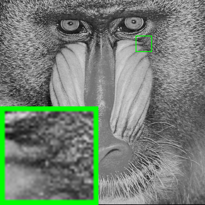
\includegraphics[width=1\textwidth]{images/twsc/awgn/resize_br_baboon.png}}
{\footnotesize Clean}
\end{minipage}
\begin{minipage}[t]{0.19\textwidth}
\centering
\raisebox{-0.15cm}{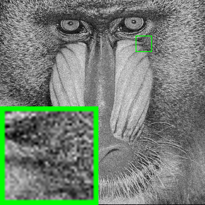
\includegraphics[width=1\textwidth]{images/twsc/awgn/resize_br_20_baboon.png}}
{\footnotesize Noisy: 22.11}
\end{minipage}
\begin{minipage}[t]{0.19\textwidth}
\centering
\raisebox{-0.15cm}{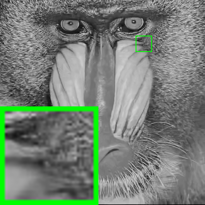
\includegraphics[width=1\textwidth]{images/twsc/awgn/resize_br_BM3D_20_baboon.png}}
{\footnotesize BM3D: 26.61}
\end{minipage}
\begin{minipage}[t]{0.19\textwidth}
\centering
\raisebox{-0.15cm}{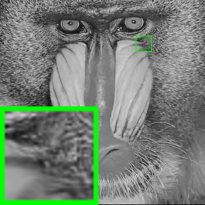
\includegraphics[width=1\textwidth]{images/twsc/awgn/resize_br_LSSC_20_baboon.png}}
{\footnotesize LSSC: 26.75}
\end{minipage}
\begin{minipage}[t]{0.19\textwidth}
\centering
\raisebox{-0.15cm}{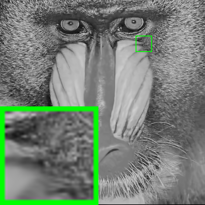
\includegraphics[width=1\textwidth]{images/twsc/awgn/resize_br_NCSR_20_baboon.png}}
{\footnotesize NCSR: 26.64}
\end{minipage}
}\vspace{-4mm}
\subfigure{
\begin{minipage}[t]{0.19\textwidth}
\centering
\raisebox{-0.15cm}{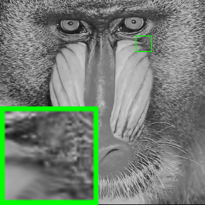
\includegraphics[width=1\textwidth]{images/twsc/awgn/resize_br_WNNM_20_baboon.png}}
{\footnotesize WNNM: 26.84}
\end{minipage}
\begin{minipage}[t]{0.19\textwidth}
\centering
\raisebox{-0.15cm}{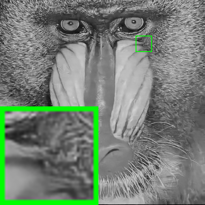
\includegraphics[width=1\textwidth]{images/twsc/awgn/resize_br_TNRD_20_baboon.png}}
{\footnotesize TNRD: 26.95}
\end{minipage}
\begin{minipage}[t]{0.19\textwidth}
\centering
\raisebox{-0.15cm}{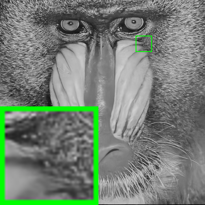
\includegraphics[width=1\textwidth]{images/twsc/awgn/resize_br_DnCNN_20_baboon.png}}
{\footnotesize DnCNN: 27.04}
\end{minipage}
\begin{minipage}[t]{0.19\textwidth}
\centering
\raisebox{-0.15cm}{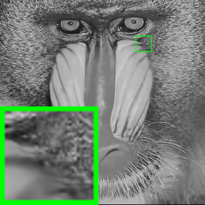
\includegraphics[width=1\textwidth]{images/twsc/awgn/resize_br_WSC_20_baboon.png}}
{\footnotesize WSC: 26.58}
\end{minipage}
\begin{minipage}[t]{0.19\textwidth}
\centering
\raisebox{-0.15cm}{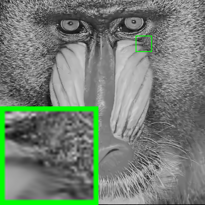
\includegraphics[width=1\textwidth]{images/twsc/awgn/resize_br_WLSWSC_20_baboon.png}}
{\footnotesize TWSC: 26.72}
\end{minipage}
}
\caption{Denoised images and PSNR (dB) results of \textsl{Baboon} by different methods (the standard deviation of noise is $\sigma=20$).}
    \label{fig5-2}
\end{adjustwidth}
\end{figure}



\begin{figure}
\begin{adjustwidth}{-2cm}{}
    \centering
\subfigure{
\begin{minipage}[t]{0.19\textwidth}
\centering
\raisebox{-0.15cm}{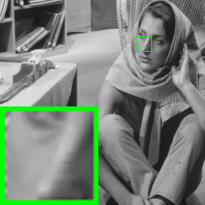
\includegraphics[width=1\textwidth]{images/twsc/awgn/resize_br_barbara.png}}
{\footnotesize Clean}
\end{minipage}
\begin{minipage}[t]{0.19\textwidth}
\centering
\raisebox{-0.15cm}{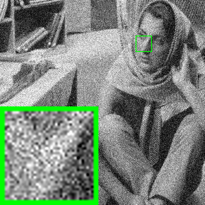
\includegraphics[width=1\textwidth]{images/twsc/awgn/resize_br_40_barbara.png}}
{\footnotesize Noisy: 16.09}
\end{minipage}
\begin{minipage}[t]{0.19\textwidth}
\centering
\raisebox{-0.15cm}{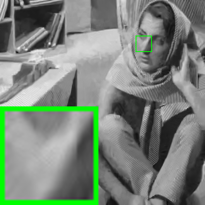
\includegraphics[width=1\textwidth]{images/twsc/awgn/resize_br_BM3D_40_barbara.png}}
{\footnotesize BM3D: 27.99}
\end{minipage}
\begin{minipage}[t]{0.19\textwidth}
\centering
\raisebox{-0.15cm}{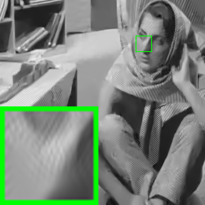
\includegraphics[width=1\textwidth]{images/twsc/awgn/resize_br_LSSC_40_barbara.png}}
{\footnotesize LSSC: 28.17}
\end{minipage}
\begin{minipage}[t]{0.19\textwidth}
\centering
\raisebox{-0.15cm}{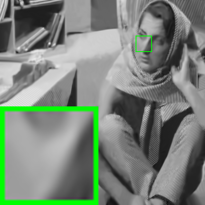
\includegraphics[width=1\textwidth]{images/twsc/awgn/resize_br_NCSR_40_barbara.png}}
{\footnotesize NCSR: 28.19}
\end{minipage}
}\vspace{-4mm}
\subfigure{
\begin{minipage}[t]{0.19\textwidth}
\centering
\raisebox{-0.15cm}{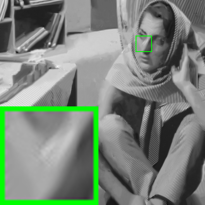
\includegraphics[width=1\textwidth]{images/twsc/awgn/resize_br_WNNM_40_barbara.png}}
{\footnotesize WNNM: 28.76}
\end{minipage}
\begin{minipage}[t]{0.19\textwidth}
\centering
\raisebox{-0.15cm}{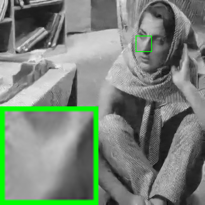
\includegraphics[width=1\textwidth]{images/twsc/awgn/resize_br_TNRD_40_barbara.png}}
{\footnotesize TNRD: 27.11}
\end{minipage}
\begin{minipage}[t]{0.19\textwidth}
\centering
\raisebox{-0.15cm}{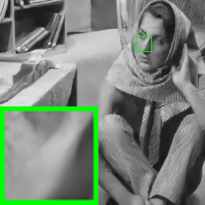
\includegraphics[width=1\textwidth]{images/twsc/awgn/resize_br_DnCNN_40_barbara.png}}
{\footnotesize DnCNN: 27.36}
\end{minipage}
\begin{minipage}[t]{0.19\textwidth}
\centering
\raisebox{-0.15cm}{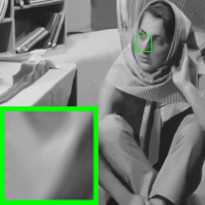
\includegraphics[width=1\textwidth]{images/twsc/awgn/resize_br_WSC_40_barbara.png}}
{\footnotesize WSC: 28.42}
\end{minipage}
\begin{minipage}[t]{0.19\textwidth}
\centering
\raisebox{-0.15cm}{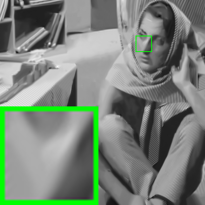
\includegraphics[width=1\textwidth]{images/twsc/awgn/resize_br_WLSWSC_40_barbara.png}}
{\footnotesize TWSC: 28.89}
\end{minipage}
}
\caption{Denoised images and PSNR (dB) results of \textsl{Barbara} by different methods (the standard deviation of noise is $\sigma=40$).}
    \label{fig5-3}
\end{adjustwidth}
\end{figure}


\begin{figure}
\begin{adjustwidth}{-2cm}{}
    \centering
\subfigure{
\begin{minipage}[t]{0.19\textwidth}
\centering
\raisebox{-0.15cm}{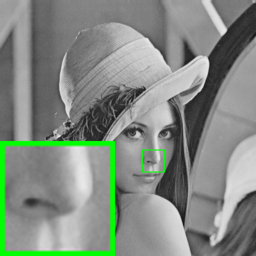
\includegraphics[width=1\textwidth]{images/twsc/awgn/resize_br_lena.png}}
{\footnotesize Clean}
\end{minipage}
\begin{minipage}[t]{0.19\textwidth}
\centering
\raisebox{-0.15cm}{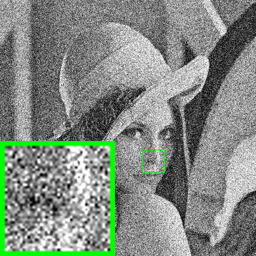
\includegraphics[width=1\textwidth]{images/twsc/awgn/resize_br_60_lena.png}}
{\footnotesize Noisy: 12.57}
\end{minipage}
\begin{minipage}[t]{0.19\textwidth}
\centering
\raisebox{-0.15cm}{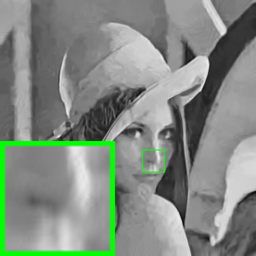
\includegraphics[width=1\textwidth]{images/twsc/awgn/resize_br_BM3D_60_lena.png}}
{\footnotesize BM3D: 28.27}
\end{minipage}
\begin{minipage}[t]{0.19\textwidth}
\centering
\raisebox{-0.15cm}{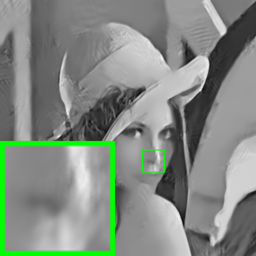
\includegraphics[width=1\textwidth]{images/twsc/awgn/resize_br_LSSC_60_lena.png}}
{\footnotesize LSSC: 28.14}
\end{minipage}
\begin{minipage}[t]{0.19\textwidth}
\centering
\raisebox{-0.15cm}{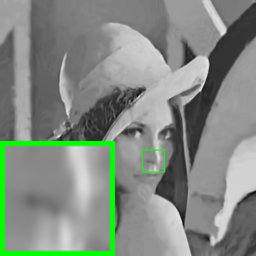
\includegraphics[width=1\textwidth]{images/twsc/awgn/resize_br_NCSR_60_lena.png}}
{\footnotesize NCSR: 28.00}
\end{minipage}
}\vspace{-4mm}
\subfigure{
\begin{minipage}[t]{0.19\textwidth}
\centering
\raisebox{-0.15cm}{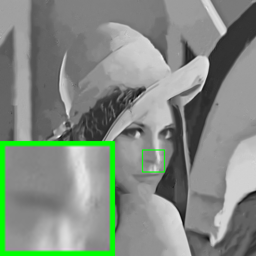
\includegraphics[width=1\textwidth]{images/twsc/awgn/resize_br_WNNM_60_lena.png}}
{\footnotesize WNNM: 28.40}
\end{minipage}
\begin{minipage}[t]{0.19\textwidth}
\centering
\raisebox{-0.15cm}{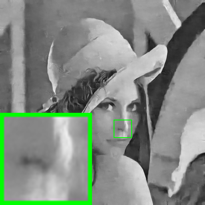
\includegraphics[width=1\textwidth]{images/twsc/awgn/resize_br_TNRD_60_lena.png}}
{\footnotesize TNRD: 28.11}
\end{minipage}
\begin{minipage}[t]{0.19\textwidth}
\centering
\raisebox{-0.15cm}{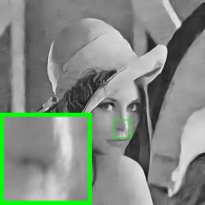
\includegraphics[width=1\textwidth]{images/twsc/awgn/resize_br_DnCNN_60_lena.png}}
{\footnotesize DnCNN: 28.53}
\end{minipage}
\begin{minipage}[t]{0.19\textwidth}
\centering
\raisebox{-0.15cm}{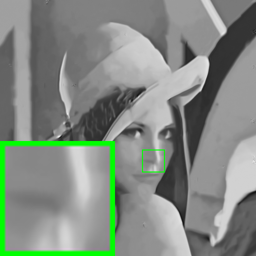
\includegraphics[width=1\textwidth]{images/twsc/awgn/resize_br_WSC_60_lena.png}}
{\footnotesize WSC: 28.07}
\end{minipage}
\begin{minipage}[t]{0.19\textwidth}
\centering
\raisebox{-0.15cm}{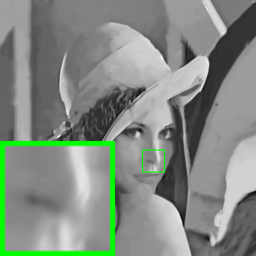
\includegraphics[width=1\textwidth]{images/twsc/awgn/resize_br_WLSWSC_60_lena.png}}
{\footnotesize TWSC: 28.48}
\end{minipage}
}
\caption{Denoised images and PSNR (dB) results of \textsl{Lena} by different methods (the standard deviation of noise is $\sigma=60$).}
    \label{fig5-4}
\end{adjustwidth}
\end{figure}

\begin{figure}
\begin{adjustwidth}{-2cm}{}
    \centering
    \begin{subfigure}[t]{0.19\textwidth}
        \centering
        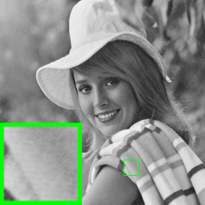
\includegraphics[width=1\textwidth]{images/twsc/awgn/resize_br_elaine.png}
	   \caption{Ground Truth}
    \end{subfigure}
    \hfill
    \begin{subfigure}[t]{0.19\textwidth}
        \centering
        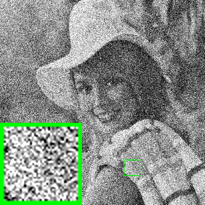
\includegraphics[width=1\textwidth]{images/twsc/awgn/resize_br_80_elaine.png}
		\caption{Noisy: 10.07}
    \end{subfigure}
    \hfill
    \begin{subfigure}[t]{0.19\textwidth}
        \centering
        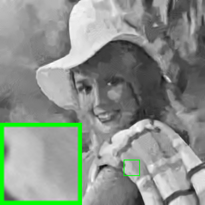
\includegraphics[width=1\textwidth]{images/twsc/awgn/resize_br_BM3D_80_elaine.png}
		\caption{BM3D: 27.16}
    \end{subfigure}
    \hfill
    \begin{subfigure}[t]{0.19\textwidth}
        \centering
        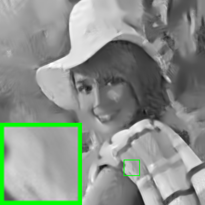
\includegraphics[width=1\textwidth]{images/twsc/awgn/resize_br_LSSC_80_elaine.png}
		\caption{LSSC: 27.02}
    \end{subfigure}
    \hfill
    \begin{subfigure}[t]{0.19\textwidth}
        \centering
        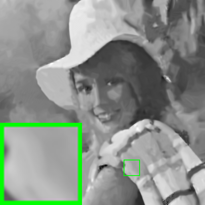
\includegraphics[width=1\textwidth]{images/twsc/awgn/resize_br_NCSR_80_elaine.png}
		\caption{NCSR: 26.88}
    \end{subfigure}
    \hfill
    \begin{subfigure}[t]{0.19\textwidth}
        \centering
        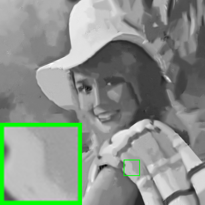
\includegraphics[width=1\textwidth]{images/twsc/awgn/resize_br_WNNM_80_elaine.png}
		\caption{WNNM: 27.26}
    \end{subfigure}
    \hfill
    \begin{subfigure}[t]{0.19\textwidth}
        \centering
        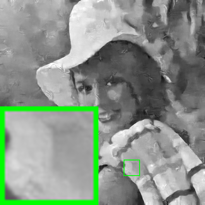
\includegraphics[width=1\textwidth]{images/twsc/awgn/resize_br_TNRD_80_elaine.png}
		\caption{TNRD: 26.35}
    \end{subfigure}
    \hfill
    \begin{subfigure}[t]{0.19\textwidth}
        \centering
        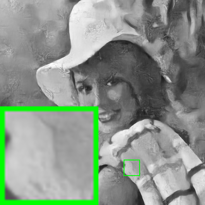
\includegraphics[width=1\textwidth]{images/twsc/awgn/resize_br_DnCNN_80_elaine.png}
		\caption{DnCNN: 26.72}
    \end{subfigure}
    \hfill
    \begin{subfigure}[t]{0.19\textwidth}
        \centering
        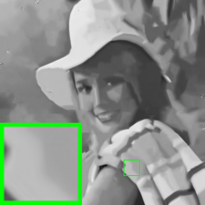
\includegraphics[width=1\textwidth]{images/twsc/awgn/resize_br_WSC_80_elaine.png}
		\caption{WSC: 27.07}
    \end{subfigure}
    \hfill
    \begin{subfigure}[t]{0.19\textwidth}
        \centering
        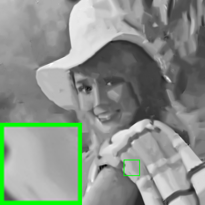
\includegraphics[width=1\textwidth]{images/twsc/awgn/resize_br_WLSWSC_80_elaine.png}
		\caption{TWSC: 27.43}
    \end{subfigure}
    \caption{Denoised images and PSNR (dB) results of \textsl{Elaine} by different methods (the standard deviation of noise is $\sigma=80$).}
    \label{fig5-5}
\end{adjustwidth}
\end{figure}

\begin{figure}
\begin{adjustwidth}{-2cm}{}
    \centering
    \begin{subfigure}[t]{0.19\textwidth}
        \centering
        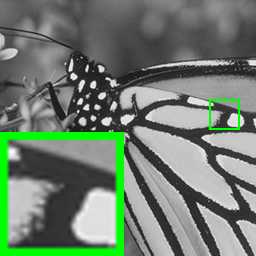
\includegraphics[width=1\textwidth]{images/twsc/awgn/br_monarch.png}
	   \caption{Ground Truth}
    \end{subfigure}
    \hfill
    \begin{subfigure}[t]{0.19\textwidth}
        \centering
        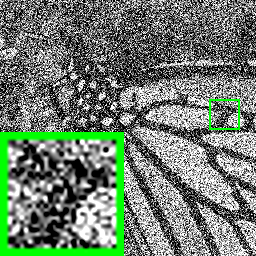
\includegraphics[width=1\textwidth]{images/twsc/awgn/br_100_monarch.png}
		\caption{Noisy: 8.10}
    \end{subfigure}
    \hfill
    \begin{subfigure}[t]{0.19\textwidth}
        \centering
        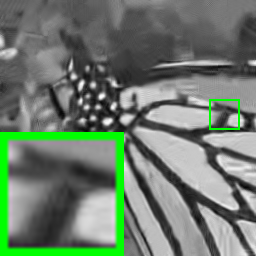
\includegraphics[width=1\textwidth]{images/twsc/awgn/br_BM3D_100_monarch.png}
		\caption{BM3D: 22.52}
    \end{subfigure}
    \hfill
    \begin{subfigure}[t]{0.19\textwidth}
        \centering
        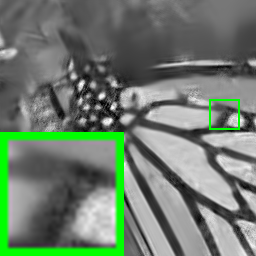
\includegraphics[width=1\textwidth]{images/twsc/awgn/br_LSSC_100_monarch.png}
		\caption{LSSC: 22.24}
    \end{subfigure}
    \hfill
    \begin{subfigure}[t]{0.19\textwidth}
        \centering
        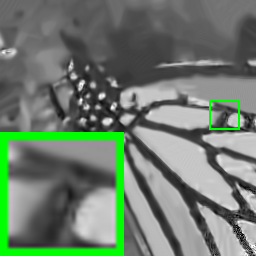
\includegraphics[width=1\textwidth]{images/twsc/awgn/br_NCSR_100_monarch.png}
		\caption{NCSR: 22.13}
    \end{subfigure}
    \hfill
    \begin{subfigure}[t]{0.19\textwidth}
        \centering
        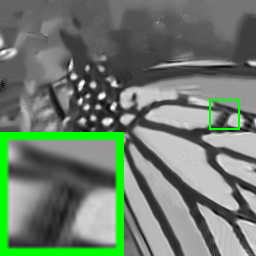
\includegraphics[width=1\textwidth]{images/twsc/awgn/br_WNNM_100_monarch.png}
		\caption{WNNM: 22.95}
    \end{subfigure}
    \hfill
    \begin{subfigure}[t]{0.19\textwidth}
        \centering
        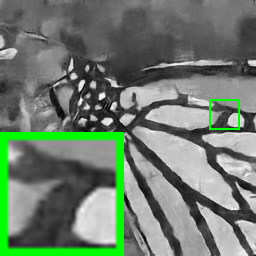
\includegraphics[width=1\textwidth]{images/twsc/awgn/br_TNRD_100_monarch.png}
		\caption{TNRD: 21.72}
    \end{subfigure}
    \hfill
    \begin{subfigure}[t]{0.19\textwidth}
        \centering
        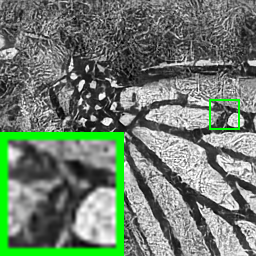
\includegraphics[width=1\textwidth]{images/twsc/awgn/br_DnCNN_100_monarch.png}
		\caption{DnCNN: 17.13}
    \end{subfigure}
    \hfill
    \begin{subfigure}[t]{0.19\textwidth}
        \centering
        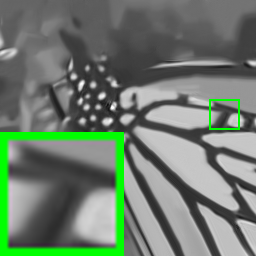
\includegraphics[width=1\textwidth]{images/twsc/awgn/br_WSC_100_monarch.png}
		\caption{WSC: 22.56}
    \end{subfigure}
    \hfill
    \begin{subfigure}[t]{0.19\textwidth}
        \centering
        \includegraphics[width=1\textwidth]{images/twsc/awgn/br_WLSWSC_100_monarch.png}
		\caption{TWSC: 23.01}
    \end{subfigure}
    \caption{Denoised images and PSNR (dB) results of \textsl{Monarch} by different methods (the standard deviation of noise is $\sigma=100$).}
    \label{fig5-6}
\end{adjustwidth}
\end{figure}




\subsection{Results on Realistic Noise Removal}


We evaluate the proposed method on two real noisy image datasets, where the images were captured under indoor and outdoor lighting conditions by different types of cameras and camera settings. 

\textbf{Dataset 1} is provided in \cite{ncwebsite}, which includes 20 real noisy images collected under uncontrolled environment.\ Since there is no ``ground truth'' of the noisy images, we only compare the visual quality of the denoised images by different methods. Fig. \ref{fig3-3} shows some sample images of this dataset.

\textbf{Dataset 2} is provided in \cite{crosschannel2016}, which includes noisy images of 11 static scenes.\ The noisy images were collected under controlled indoor environment.\ Each scene was shot 500 times under the same camera and camera setting.\ The mean image of the 500 shots is roughly taken as the ``ground truth'', with which the PSNR and SSIM \cite{ssim} can be computed. 15 images of size $512\times512$ were cropped in \cite{crosschannel2016} to evaluate the different denoising methods. Fig. \ref{fig3-4} shows some sample images of this dataset.


We compare the proposed TWSC method with CBM3D \cite{cbm3d}, WNNM \cite{wnnm}, TNRD \cite{tnrd}, DnCNN \cite{dncnn}, the commercial software Neat Image (NI) \cite{neatimage}, the state-of-the-art real image denoising methods ``Noise Clinic'' (NC) \cite{noiseclinic} and CC \cite{crosschannel2016}. Since WNNM and TNRD are designed for gray level images, we applied them to each channel of real noisy images. The input noise stds $\sigma_{c}$ ($c\in\{r,g,b\}$) for WNNM are estimated by a noise estimation method \cite{Chen2015ICCV}. TNRD achieves its best results when setting the noise std of the trained models at $\sigma_{c}=10$. The methods of CBM3D and DnCNN can directly deal with color images, and the input noise std is set as $\sigma=\sqrt{(\sigma_{r}^{2}+\sigma_{g}^{2}+\sigma_{b}^{2})/3}$.\ Due to limited space, we do not compare with the baseline method WSC on visual quality.

\textbf{Results on Dataset 1}. Fig. \ref{fig5-7} show the denoised images of ``Dog''. (The method CC \cite{crosschannel2016} is not compared since its code is not available.) One can see that CBM3D and WNNM tend to over-smooth the image.\ DnCNN, TNRD and NI remain many noise-caused color artifacts across the whole image. NC is better than other methods except the proposed TWSC. These results demonstrate that the methods designed for AWGN are not effective for realistic noise removal.\ Though NC and NI methods are specifically developed for real noisy images, their performance is not satisfactory.\ In comparison, the proposed TWSC works much better in removing the noise while maintaining the details (see the zoom-in window in ``Dog'') than the other competing methods.\ More visual comparisons can be found in the Figures \ref{fig5-8}-\ref{fig5-10}, in which we can see that our proposed method performs better than the competing methods.

\textbf{Results on Dataset 2}. The average PSNR and SSIM results on the 15 cropped images by competing methods are listed in Table \ref{tab5-2}. One can see that the proposed TWSC is much better than other competing methods, including CC and the baseline method WSC. Fig. \ref{fig5-11} shows the denoised images of a scene captured by Canon 5D Mark 3 at ISO = 3200. One can see that the proposed TWSC method results in not only higher PSNR and SSIM measures, but also much better visual quality than the other denoising methods. More comparisons can be found in Figures \ref{fig5-12}--\ref{fig5-15}, our proposed TWSC method achieves better performance than the the competing methods.


\begin{table}[hbp]
\caption{Average results on PSNR(dB) and SSIM of different denoising methods on 15 cropped real noisy images used in \cite{crosschannel2016}.}
\label{tab5-2}
\begin{center}
\renewcommand\arraystretch{1}
\scriptsize
\begin{tabular*}{1\textwidth}{@{\extracolsep{\fill}}ccccccccccc}
\hline
Metric
&
\textbf{CBM3D}
&
\textbf{WNNM}
&
\textbf{TNRD}
&
\textbf{DnCNN}
&
\textbf{NI}
&
\textbf{NC}
&
\textbf{CC}
&
\textbf{WSC}
&
\textbf{TWSC}
\\
\hline
PSNR & 35.19 & 35.77 & 36.61 & 33.86 & 35.49 & 36.43  & 36.88 & 37.36 & \textbf{37.81}
\\
\hline
SSIM & 0.9063 & 0.9381 & 0.9463 & 0.8635 & 0.9126 & 0.9364 & 0.9481 & 0.9516 & \textbf{0.9586}
\\
\hline
\end{tabular*}
\end{center}
\end{table}

%% --------------------NC------------

\begin{figure}
    \centering
    \begin{subfigure}[t]{0.24\textwidth}
        \centering
        \includegraphics[width=1\textwidth]{images/twsc/nc/resize_br_Noisy_dog.png}
		\caption{Noisy}
    \end{subfigure}
    \hfill
    \begin{subfigure}[t]{0.24\textwidth}
        \centering
        \includegraphics[width=1\textwidth]{images/twsc/nc/resize_br_CBM3D_dog.png}
		\caption{CBM3D}
    \end{subfigure}
    \hfill
    \begin{subfigure}[t]{0.24\textwidth}
        \centering
        \includegraphics[width=1\textwidth]{images/twsc/nc/resize_br_WNNM_dog.png}
\caption{WNNM}
    \end{subfigure}
    \hfill
    \begin{subfigure}[t]{0.24\textwidth}
        \centering
        \includegraphics[width=1\textwidth]{images/twsc/nc/resize_br_TRD_dog.png}
\caption{TNRD}
    \end{subfigure}
    \hfill
    \begin{subfigure}[t]{0.24\textwidth}
        \centering
        \includegraphics[width=1\textwidth]{images/twsc/nc/resize_br_DnCNN_dog.png}
\caption{DnCNN}
    \end{subfigure}
\hfill
    \begin{subfigure}[t]{0.24\textwidth}
        \centering
        \includegraphics[width=1\textwidth]{images/twsc/nc/resize_br_NI_dog.png}
\caption{NI}
    \end{subfigure}
\hfill
    \begin{subfigure}[t]{0.24\textwidth}
        \centering
        \includegraphics[width=1\textwidth]{images/twsc/nc/resize_br_NC_dog.png}
		\caption{NC}
    \end{subfigure}
    \hfill
    \begin{subfigure}[t]{0.24\textwidth}
        \centering
        \includegraphics[width=1\textwidth]{images/twsc/nc/resize_br_TWSC_dog.png}
		\caption{TWSC}
    \end{subfigure}
    \caption{Denoised images of the real noisy image \textsl{Dog} \cite{ncwebsite} by different methods.\ The estimated noise levels of R, G, and B channels are 16.8, 17.0, and 16.6, respectively.\ The images are better to be zoomed in on screen.}
    \label{fig5-7}
\end{figure}


\begin{figure}
    \centering
    \begin{subfigure}[t]{0.24\textwidth}
        \centering
        \includegraphics[width=1\textwidth]{images/twsc/nc/resize_br_Noisy_bears.png}
		\caption{Noisy}
    \end{subfigure}
    \hfill
    \begin{subfigure}[t]{0.24\textwidth}
        \centering
        \includegraphics[width=1\textwidth]{images/twsc/nc/resize_br_CBM3D_bears.png}
		\caption{CBM3D}
    \end{subfigure}
    \hfill
    \begin{subfigure}[t]{0.24\textwidth}
        \centering
        \includegraphics[width=1\textwidth]{images/twsc/nc/resize_br_WNNM_bears.png}
\caption{WNNM}
    \end{subfigure}
    \hfill
    \begin{subfigure}[t]{0.24\textwidth}
        \centering
        \includegraphics[width=1\textwidth]{images/twsc/nc/resize_br_TRD_bears.png}
\caption{TNRD}
    \end{subfigure}
    \hfill
    \begin{subfigure}[t]{0.24\textwidth}
        \centering
        \includegraphics[width=1\textwidth]{images/twsc/nc/resize_br_DnCNN_bears.png}
\caption{DnCNN}
    \end{subfigure}
\hfill
    \begin{subfigure}[t]{0.24\textwidth}
        \centering
        \includegraphics[width=1\textwidth]{images/twsc/nc/resize_br_NI_bears.png}
\caption{NI}
    \end{subfigure}
\hfill
    \begin{subfigure}[t]{0.24\textwidth}
        \centering
        \includegraphics[width=1\textwidth]{images/twsc/nc/resize_br_NC_bears.png}
		\caption{NC}
    \end{subfigure}
    \hfill
    \begin{subfigure}[t]{0.24\textwidth}
        \centering
        \includegraphics[width=1\textwidth]{images/twsc/nc/resize_br_TWSC_bears.png}
		\caption{TWSC}
    \end{subfigure}
    \caption{Denoised images of the real noisy image \textsl{Bears} \cite{ncwebsite} by different methods.\ The estimated noise levels of R, G, and B channels are ?, ?, and ?, respectively.\ The images are better to be zoomed in on screen.}
    \label{fig5-8}
\end{figure}


\begin{figure}
    \centering
    \begin{subfigure}[t]{0.24\textwidth}
        \centering
        \includegraphics[width=1\textwidth]{images/twsc/nc/resize_br_Noisy_frog.png}
		\caption{Noisy}
    \end{subfigure}
    \hfill
    \begin{subfigure}[t]{0.24\textwidth}
        \centering
        \includegraphics[width=1\textwidth]{images/twsc/nc/resize_br_CBM3D_frog.png}
		\caption{CBM3D}
    \end{subfigure}
    \hfill
    \begin{subfigure}[t]{0.24\textwidth}
        \centering
        \includegraphics[width=1\textwidth]{images/twsc/nc/resize_br_WNNM_frog.png}
\caption{WNNM}
    \end{subfigure}
    \hfill
    \begin{subfigure}[t]{0.24\textwidth}
        \centering
        \includegraphics[width=1\textwidth]{images/twsc/nc/resize_br_TRD_frog.png}
\caption{TNRD}
    \end{subfigure}
    \hfill
    \begin{subfigure}[t]{0.24\textwidth}
        \centering
        \includegraphics[width=1\textwidth]{images/twsc/nc/resize_br_DnCNN_frog.png}
\caption{DnCNN}
    \end{subfigure}
\hfill
    \begin{subfigure}[t]{0.24\textwidth}
        \centering
        \includegraphics[width=1\textwidth]{images/twsc/nc/resize_br_NI_frog.png}
\caption{NI}
    \end{subfigure}
\hfill
    \begin{subfigure}[t]{0.24\textwidth}
        \centering
        \includegraphics[width=1\textwidth]{images/twsc/nc/resize_br_NC_frog.png}
		\caption{NC}
    \end{subfigure}
    \hfill
    \begin{subfigure}[t]{0.24\textwidth}
        \centering
        \includegraphics[width=1\textwidth]{images/twsc/nc/resize_br_TWSC_frog.png}
		\caption{TWSC}
    \end{subfigure}
    \caption{Denoised images of the real noisy image \textsl{Frog} \cite{ncwebsite} by different methods.\ The estimated noise levels of R, G, and B channels are ?, ?, and ?, respectively.\ The images are better to be zoomed in on screen.}
    \label{fig5-9}
\end{figure}


\begin{figure}
    \centering
    \begin{subfigure}[t]{0.24\textwidth}
        \centering
        \includegraphics[width=1\textwidth]{images/twsc/nc/resize_br_Noisy_chinesegirl.png}
		\caption{Noisy}
    \end{subfigure}
    \hfill
    \begin{subfigure}[t]{0.24\textwidth}
        \centering
        \includegraphics[width=1\textwidth]{images/twsc/nc/resize_br_CBM3D_chinesegirl.png}
		\caption{CBM3D}
    \end{subfigure}
    \hfill
    \begin{subfigure}[t]{0.24\textwidth}
        \centering
        \includegraphics[width=1\textwidth]{images/twsc/nc/resize_br_WNNM_chinesegirl.png}
\caption{WNNM}
    \end{subfigure}
    \hfill
    \begin{subfigure}[t]{0.24\textwidth}
        \centering
        \includegraphics[width=1\textwidth]{images/twsc/nc/resize_br_TRD_chinesegirl.png}
\caption{TNRD}
    \end{subfigure}
    \hfill
    \begin{subfigure}[t]{0.24\textwidth}
        \centering
        \includegraphics[width=1\textwidth]{images/twsc/nc/resize_br_DnCNN_chinesegirl.png}
\caption{DnCNN}
    \end{subfigure}
\hfill
    \begin{subfigure}[t]{0.24\textwidth}
        \centering
        \includegraphics[width=1\textwidth]{images/twsc/nc/resize_br_NI_chinesegirl.png}
\caption{NI}
    \end{subfigure}
\hfill
    \begin{subfigure}[t]{0.24\textwidth}
        \centering
        \includegraphics[width=1\textwidth]{images/twsc/nc/resize_br_NC_chinesegirl.png}
		\caption{NC}
    \end{subfigure}
    \hfill
    \begin{subfigure}[t]{0.24\textwidth}
        \centering
        \includegraphics[width=1\textwidth]{images/twsc/nc/resize_br_TWSC_chinesegirl.png}
		\caption{TWSC}
    \end{subfigure}
    \caption{Denoised images of the real noisy image \textsl{Girl} \cite{ncwebsite} by different methods.\ The estimated noise levels of R, G, and B channels are ?, ?, and ?, respectively.\ The images are better to be zoomed in on screen.}
    \label{fig5-10}
\end{figure}


%%---------------------------CC--------------------------
\begin{figure}
    \centering
    \begin{subfigure}[t]{0.19\textwidth}
        \centering
        \includegraphics[width=1\textwidth]{images/twsc/cc/resize_br_Mean_5dmark3_iso3200_1_real.png}
		\caption{Mean Image}
    \end{subfigure}
    \hfill
    \begin{subfigure}[t]{0.19\textwidth}
        \centering
        \includegraphics[width=1\textwidth]{images/twsc/cc/resize_br_Noisy_5dmark3_iso3200_1_real.png}
		\caption{Noisy 37.00}
    \end{subfigure}
    \hfill
    \begin{subfigure}[t]{0.19\textwidth}
        \centering
        \includegraphics[width=1\textwidth]{images/twsc/cc/resize_br_CBM3D_5dmark3_iso3200_1_real.png}
		\caption{CBM3D 39.72}
    \end{subfigure}
    \hfill
    \begin{subfigure}[t]{0.19\textwidth}
        \centering
        \includegraphics[width=1\textwidth]{images/twsc/cc/resize_br_WNNM_5dmark3_iso3200_1_real.png}
\caption{WNNM 37.48}
    \end{subfigure}
    \hfill
    \begin{subfigure}[t]{0.19\textwidth}
        \centering
        \includegraphics[width=1\textwidth]{images/twsc/cc/resize_br_TRD_5dmark3_iso3200_1_real.png}
\caption{TNRD 39.46}
    \end{subfigure}
    \hfill
    \begin{subfigure}[t]{0.19\textwidth}
        \centering
        \includegraphics[width=1\textwidth]{images/twsc/cc/resize_br_DnCNN_5dmark3_iso3200_1_real.png}
\caption{DnCNN 37.26}
    \end{subfigure}
\hfill
    \begin{subfigure}[t]{0.19\textwidth}
        \centering
        \includegraphics[width=1\textwidth]{images/twsc/cc/resize_br_NI_5dmark3_iso3200_1_real.png}
\caption{NI 37.68}
    \end{subfigure}
\hfill
    \begin{subfigure}[t]{0.19\textwidth}
        \centering
        \includegraphics[width=1\textwidth]{images/twsc/cc/resize_br_NC_5dmark3_iso3200_1_real.png}
		\caption{NC 38.76}
    \end{subfigure}
    \hfill
    \begin{subfigure}[t]{0.19\textwidth}
        \centering
        \includegraphics[width=1\textwidth]{images/twsc/cc/resize_br_CCNoise_5dmark3_iso3200_1.png}
		\caption{CC 38.37}
    \end{subfigure}
    \hfill
    \begin{subfigure}[t]{0.19\textwidth}
        \centering
        \includegraphics[width=1\textwidth]{images/twsc/cc/resize_br_TWSC_5dmark3_iso3200_1.png}
		\caption{TWSC \textbf{40.75}}
    \end{subfigure}
    \caption{Denoised images and PSNR (dB) results of the real noisy image \textsl{Canon 5D Mark 3 ISO 3200 1} \cite{crosschannel2016} by different methods.\ The estimated noise levels of R, G, and B channels are 1.6, 1.5, and 1.6, respectively.\ The images are better to be zoomed in on screen.}
    \label{fig5-11}
\end{figure}


\begin{figure}
    \centering
    \begin{subfigure}[t]{0.19\textwidth}
        \centering
        \includegraphics[width=1\textwidth]{images/twsc/cc/resize_br_Mean_d600_iso3200_2_real.png}
		\caption{Mean Image}
    \end{subfigure}
    \hfill
    \begin{subfigure}[t]{0.19\textwidth}
        \centering
        \includegraphics[width=1\textwidth]{images/twsc/cc/resize_br_Noisy_d600_iso3200_2_real.png}
		\caption{Noisy 33.77}
    \end{subfigure}
    \hfill
    \begin{subfigure}[t]{0.19\textwidth}
        \centering
        \includegraphics[width=1\textwidth]{images/twsc/cc/resize_br_CBM3D_d600_iso3200_2_real.png}
		\caption{CBM3D 35.06}
    \end{subfigure}
    \hfill
    \begin{subfigure}[t]{0.19\textwidth}
        \centering
        \includegraphics[width=1\textwidth]{images/twsc/cc/resize_br_WNNM_d600_iso3200_2_real.png}
\caption{WNNM 36.07}
    \end{subfigure}
    \hfill
    \begin{subfigure}[t]{0.19\textwidth}
        \centering
        \includegraphics[width=1\textwidth]{images/twsc/cc/resize_br_TRD_d600_iso3200_2_real.png}
\caption{TNRD 36.34}
    \end{subfigure}
    \hfill
    \begin{subfigure}[t]{0.19\textwidth}
        \centering
        \includegraphics[width=1\textwidth]{images/twsc/cc/resize_br_DnCNN_d600_iso3200_2_real.png}
\caption{DnCNN 34.48}
    \end{subfigure}
\hfill
    \begin{subfigure}[t]{0.19\textwidth}
        \centering
        \includegraphics[width=1\textwidth]{images/twsc/cc/resize_br_NI_d600_iso3200_2_real.png}
\caption{NI 35.36}
    \end{subfigure}
\hfill
    \begin{subfigure}[t]{0.19\textwidth}
        \centering
        \includegraphics[width=1\textwidth]{images/twsc/cc/resize_br_NC_d600_iso3200_2_real.png}
		\caption{NC 36.70}
    \end{subfigure}
    \hfill
    \begin{subfigure}[t]{0.19\textwidth}
        \centering
        \includegraphics[width=1\textwidth]{images/twsc/cc/resize_br_CCNoise_d600_iso3200_2.png}
		\caption{CC 35.95}
    \end{subfigure}
    \hfill
    \begin{subfigure}[t]{0.19\textwidth}
        \centering
        \includegraphics[width=1\textwidth]{images/twsc/cc/resize_br_TWSC_d600_iso3200_2.png}
		\caption{TWSC \textbf{37.07}}
    \end{subfigure}
    \caption{Denoised images and PSNR (dB) results of the real noisy image \textsl{Nikon D600 ISO 3200 2} \cite{crosschannel2016} by different methods.\ The estimated noise levels of R, G, and B channels are 1.2, 1.3, and 1.4, respectively.\ The images are better to be zoomed in on screen.}
    \label{fig5-12}
\end{figure}


\begin{figure}
    \centering
    \begin{subfigure}[t]{0.19\textwidth}
        \centering
        \includegraphics[width=1\textwidth]{images/twsc/cc/resize_br_Mean_d800_iso1600_1_real.png}
		\caption{Mean Image}
    \end{subfigure}
    \hfill
    \begin{subfigure}[t]{0.19\textwidth}
        \centering
        \includegraphics[width=1\textwidth]{images/twsc/cc/resize_br_Noisy_d800_iso1600_1_real.png}
		\caption{Noisy 35.47}
    \end{subfigure}
    \hfill
    \begin{subfigure}[t]{0.19\textwidth}
        \centering
        \includegraphics[width=1\textwidth]{images/twsc/cc/resize_br_CBM3D_d800_iso1600_1_real.png}
		\caption{CBM3D 36.79}
    \end{subfigure}
    \hfill
    \begin{subfigure}[t]{0.19\textwidth}
        \centering
        \includegraphics[width=1\textwidth]{images/twsc/cc/resize_br_WNNM_d800_iso1600_1_real.png}
\caption{WNNM 36.33}
    \end{subfigure}
    \hfill
    \begin{subfigure}[t]{0.19\textwidth}
        \centering
        \includegraphics[width=1\textwidth]{images/twsc/cc/resize_br_TRD_d800_iso1600_1_real.png}
\caption{TNRD 38.07}
    \end{subfigure}
    \hfill
    \begin{subfigure}[t]{0.19\textwidth}
        \centering
        \includegraphics[width=1\textwidth]{images/twsc/cc/resize_br_DnCNN_d800_iso1600_1_real.png}
\caption{DnCNN 35.79}
    \end{subfigure}
\hfill
    \begin{subfigure}[t]{0.19\textwidth}
        \centering
        \includegraphics[width=1\textwidth]{images/twsc/cc/resize_br_NI_d800_iso1600_1_real.png}
\caption{NI 37.34}
    \end{subfigure}
\hfill
    \begin{subfigure}[t]{0.19\textwidth}
        \centering
        \includegraphics[width=1\textwidth]{images/twsc/cc/resize_br_NC_d800_iso1600_1_real.png}
		\caption{NC 38.01}
    \end{subfigure}
    \hfill
    \begin{subfigure}[t]{0.19\textwidth}
        \centering
        \includegraphics[width=1\textwidth]{images/twsc/cc/resize_br_CCNoise_d800_iso1600_1.png}
		\caption{CC 37.99}
    \end{subfigure}
    \hfill
    \begin{subfigure}[t]{0.19\textwidth}
        \centering
        \includegraphics[width=1\textwidth]{images/twsc/cc/resize_br_TWSC_d800_iso1600_1.png}
		\caption{TWSC \textbf{39.18}}
    \end{subfigure}
    \caption{Denoised images and PSNR (dB) results of the real noisy image \textsl{Nikon D800 ISO 1600 1} \cite{crosschannel2016} by different methods.\ The estimated noise levels of R, G, and B channels are ?, ?, and ?, respectively.\ The images are better to be zoomed in on screen.}
    \label{fig5-13}
\end{figure}


\begin{figure}
    \centering
    \begin{subfigure}[t]{0.19\textwidth}
        \centering
        \includegraphics[width=1\textwidth]{images/twsc/cc/resize_br_Mean_d800_iso3200_1_real.png}
		\caption{Mean Image}
    \end{subfigure}
    \hfill
    \begin{subfigure}[t]{0.19\textwidth}
        \centering
        \includegraphics[width=1\textwidth]{images/twsc/cc/resize_br_Noisy_d800_iso3200_1_real.png}
		\caption{Noisy 33.26}
    \end{subfigure}
    \hfill
    \begin{subfigure}[t]{0.19\textwidth}
        \centering
        \includegraphics[width=1\textwidth]{images/twsc/cc/resize_br_CBM3D_d800_iso3200_1_real.png}
		\caption{CBM3D 35.04}
    \end{subfigure}
    \hfill
    \begin{subfigure}[t]{0.19\textwidth}
        \centering
        \includegraphics[width=1\textwidth]{images/twsc/cc/resize_br_WNNM_d800_iso3200_1_real.png}
\caption{WNNM 38.56}
    \end{subfigure}
    \hfill
    \begin{subfigure}[t]{0.19\textwidth}
        \centering
        \includegraphics[width=1\textwidth]{images/twsc/cc/resize_br_TRD_d800_iso3200_1_real.png}
\caption{TNRD 37.66}
    \end{subfigure}
    \hfill
    \begin{subfigure}[t]{0.19\textwidth}
        \centering
        \includegraphics[width=1\textwidth]{images/twsc/cc/resize_br_DnCNN_d800_iso3200_1_real.png}
\caption{DnCNN 34.08}
    \end{subfigure}
\hfill
    \begin{subfigure}[t]{0.19\textwidth}
        \centering
        \includegraphics[width=1\textwidth]{images/twsc/cc/resize_br_NI_d800_iso3200_1_real.png}
\caption{NI 36.95}
    \end{subfigure}
\hfill
    \begin{subfigure}[t]{0.19\textwidth}
        \centering
        \includegraphics[width=1\textwidth]{images/twsc/cc/resize_br_NC_d800_iso3200_1_real.png}
		\caption{NC 38.07}
    \end{subfigure}
    \hfill
    \begin{subfigure}[t]{0.19\textwidth}
        \centering
        \includegraphics[width=1\textwidth]{images/twsc/cc/resize_br_CCNoise_d800_iso3200_1.png}
		\caption{CC 39.01}
    \end{subfigure}
    \hfill
    \begin{subfigure}[t]{0.19\textwidth}
        \centering
        \includegraphics[width=1\textwidth]{images/twsc/cc/resize_br_TWSC_d800_iso3200_1.png}
		\caption{TWSC \textbf{39.98}}
    \end{subfigure}
    \caption{Denoised images and PSNR (dB) results of the real noisy image \textsl{Nikon D800 ISO 3200 1} \cite{crosschannel2016} by different methods.\ The estimated noise levels of R, G, and B channels are ?, ?, and ?, respectively.\ The images are better to be zoomed in on screen.}
    \label{fig5-14}
\end{figure}



\begin{figure}
    \centering
    \begin{subfigure}[t]{0.19\textwidth}
        \centering
        \includegraphics[width=1\textwidth]{images/twsc/cc/resize_br_Mean_d800_iso6400_1_real.png}
		\caption{Mean Image}
    \end{subfigure}
    \hfill
    \begin{subfigure}[t]{0.19\textwidth}
        \centering
        \includegraphics[width=1\textwidth]{images/twsc/cc/resize_br_Noisy_d800_iso6400_1_real.png}
		\caption{Noisy 29.63}
    \end{subfigure}
    \hfill
    \begin{subfigure}[t]{0.19\textwidth}
        \centering
        \includegraphics[width=1\textwidth]{images/twsc/cc/resize_br_CBM3D_d800_iso6400_1_real.png}
		\caption{CBM3D 31.12}
    \end{subfigure}
    \hfill
    \begin{subfigure}[t]{0.19\textwidth}
        \centering
        \includegraphics[width=1\textwidth]{images/twsc/cc/resize_br_WNNM_d800_iso6400_1_real.png}
\caption{WNNM 33.27}
    \end{subfigure}
    \hfill
    \begin{subfigure}[t]{0.19\textwidth}
        \centering
        \includegraphics[width=1\textwidth]{images/twsc/cc/resize_br_TRD_d800_iso6400_1_real.png}
\caption{TNRD 32.80}
    \end{subfigure}
    \hfill
    \begin{subfigure}[t]{0.19\textwidth}
        \centering
        \includegraphics[width=1\textwidth]{images/twsc/cc/resize_br_DnCNN_d800_iso6400_1_real.png}
\caption{DnCNN 29.83}
    \end{subfigure}
\hfill
    \begin{subfigure}[t]{0.19\textwidth}
        \centering
        \includegraphics[width=1\textwidth]{images/twsc/cc/resize_br_NI_d800_iso6400_1_real.png}
\caption{NI 31.28}
    \end{subfigure}
\hfill
    \begin{subfigure}[t]{0.19\textwidth}
        \centering
        \includegraphics[width=1\textwidth]{images/twsc/cc/resize_br_NC_d800_iso6400_1_real.png}
		\caption{NC 33.49}
    \end{subfigure}
    \hfill
    \begin{subfigure}[t]{0.19\textwidth}
        \centering
        \includegraphics[width=1\textwidth]{images/twsc/cc/resize_br_CCNoise_d800_iso6400_1.png}
		\caption{CC 34.61}
    \end{subfigure}
    \hfill
    \begin{subfigure}[t]{0.19\textwidth}
        \centering
        \includegraphics[width=1\textwidth]{images/twsc/cc/resize_br_TWSC_d800_iso6400_1.png}
		\caption{TWSC \textbf{35.47}}
    \end{subfigure}
    \caption{Denoised images and PSNR (dB) results of the real noisy image \textsl{Nikon D800 ISO 6400 1} \cite{crosschannel2016} by different methods.\ The estimated noise levels of R, G, and B channels are ?, ?, and ?, respectively.\ The images are better to be zoomed in on screen.}
    \label{fig5-15}
\end{figure}



\section{Conclusion}

The realistic noise in real-world noisy images is very complex due to the various factors in digital camera pipelines, making the realistic image denoising problem much more challenging than white Gaussian noise removal.\ We proposed a novel trilateral weighted sparse coding (TWSC) scheme to exploit the noise properties across different channels and patches.\ Specifically, we introduced two weight matrices into the data term of sparse coding model to adaptively process each patch in each channel, and a weight matrix to better model image priors.\ The proposed TWSC model was solved via the ADMM algorithm and the solution existence and convergence can be guaranteed.\ Experiments demonstrated the superior performance of TWSC to the state-of-the-art denoising methods, including those methods designed for realistic noise.